\documentclass{acm_proc_article-sp}

\usepackage{pslatex}
\usepackage{epsfig}
\usepackage{appendix}
\usepackage{float}
\usepackage{url}
\usepackage{subfigure}

\floatstyle{ruled}
\newfloat{program}{thp}{lop}
\floatname{program}{Program}

\begin{document}

\title{Evaluation of a Cache-Oblivious Data Structure}

\numberofauthors{1}
\author{Maks Verver\\ \email{m.verver@student.utwente.nl}}

% Obligatory permission block   
\toappear{
Permission to make digital or hard copies of all or part of this work
for personal or classroom use is granted without fee provided that
copies are not made or distributed for profit or commercial advantage
and that copies bear this notice and the full citation on the first
page. To copy otherwise, or republish, to post on servers or to
redistribute to lists, requires prior specific permission.

\textit{\small 9$^{th}$ Twente Student Conference on IT, Enschede, June 23$^{rd}$, 2008}

Copyright 2008, University of Twente, Faculty of Electrical Engineering,
Mathematics and Computer Science}
% End of obligatory permission block

\maketitle

\begin{abstract}
In modern computer hardware architecture memory is organized in a hierarchy
consisting of several types of memory with different memory sizes, block
transfer sizes and access times.
Traditionally, data structures are evaluated in a theoretical model that
does not take the existence of a memory hierarchy into account. The
cache-oblivious model has been proposed as a more accurate model.
Although several data structures have been described in this model
relatively little empirical performance data is available.
This paper presents the results of an empirical evaluation of several data
structures in a realistic scenario and aims to provide insight into
the applicability of cache-oblivious data structures in practice.
\end{abstract}

\keywords{cache efficiency, locality of reference, algorithms}

\section{Introduction}
A fundamental part of theoretical computer science is the study of algorithms (formal descriptions of how computations may be performed) and data structures (descriptions of how information is organized and stored in computers). Traditionally, algorithms have been evaluated in a simplified model of computation. In this model it is assumed that a computer executes an algorithm in discrete steps. At each step it performs one elementary operation (e.g. comparing two numbers, adding one to another, storing a value in memory, et cetera). Each elementary operation is performed within a constant time. In this model, both storing and retrieving data values in memory is considered to be an elementary operation.

This model is close enough to the way computers work to be extremely useful in the development and analysis of data structures and algorithms that work well in practice. However, like every model, it is a simplification of reality. One of the simplifications is the assumption that data can be stored or retrieved at any location in a constant amount of time, which is why we will call this the \emph{uniform memory model}.
Advancements in software and hardware design over the last two de\-cades have caused this assumption to be increasingly detached from reality.

The main cause for this is the increasing difference between processor and memory speeds. As processor speeds have increased greatly, the time required to transfer data between processor and main memory has become a bottleneck for many types of computations. Hardware architects have added faster (but small) cache memory at various points in the computer architecture to reduce this problem.
Similar developments have taken place on the boundary between main memory and disk-based storage.

As a result, a modern computer system lacks a central memory storage with uniform performance characteristics. Instead, it employs a hierarchy of memory storage types. Figure \ref{fig-memhier} gives a typical example of such a hierarchy. The processor can directly manipulate data contained in its registers only. To access data in a lower level in the memory hierarchy, the data must be transferred upward through the memory hierarchy. Memory is typically transferred in blocks of data of a fixed size (although bulk transfers involving multiple blocks of data at once are also supported at the memory and disk level).

\begin{figure}
\centering
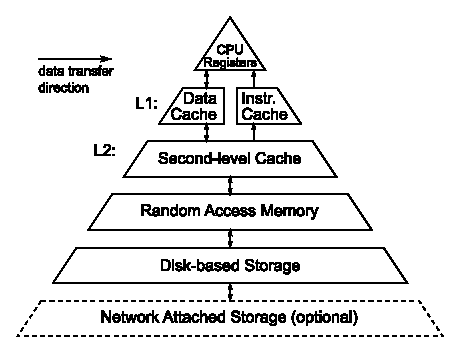
\includegraphics[width=55mm]{memhier}
\caption{Schematic depiction of the memory hierarchy}\label{fig-memhier}
\end{figure}

In the memory hierarchy, every next level of storage is both significantly slower and significantly larger than the one above it and with increasing memory sizes, the block size increases as well. Table \ref{tab-memhier} gives an overview of typical memory sizes, block sizes, and access times. The values for the (general purpose) registers, L1 cache and L2 cache are those for the Pentium M processor as given in \cite{intel-opt}; other values are approximate.

\begin{table}
\begin{center}
\begin{tabular}{ l l l l }
\hline
\textbf{Type} & \textbf{Total Size} & \textbf{Block Size} & \textbf{Access Time} \\
\hline
Registers  &   32~bytes & 4~bytes & 1 cycle \\
L1 Cache   &   32~KB    & 64~bytes & 3 cycles \\
L2 Cache   &    1~MB    & 64~bytes & 9 cycles \\
RAM        &  $\pm$ 2 GB    & 1~KB     & 50-100 cycles \\
Disk       &  $\pm$ 300 GB    & 4~KB     & 5,000-10,000 cycles \\
\hline
\end{tabular}
\caption{Sizes and access times of various types of storage}
\label{tab-memhier}
\end{center}
\end{table}

To conclude: the memory model used in real computer systems is quite a bit more complex than the uniform memory model assumed. Given this reality, the performance of many existing algorithms and data structures can be improved by taking the existence of a memory hierarchy into account. This has prompted research into new memory models that are more realistic. We will consider three classes of data structures and algorithms, depending on the assumptions that are made about the environment in their definition:
\begin{list}{}{}
\item \textbf{Cache-unaware} data structures and algorithms are designed for
the traditional uniform memory model, with no consideration of the existence
of a memory hierarchy.
\item \textbf{Cache-aware} (or \textbf{cache-conscious}) data structures and
algorithms are designed to perform optimally in the external memory model
(described below) but require parametrization with some or all properties of
the cache layout (such as block size or cache memory size).
\item \textbf{Cache-oblivious} data structures and algorithms are designed to
perform optimally in the cache-oblivious model (explained below) which does
not allow para\-metri\-zation with properties of the cache layout.
\end{list}

A great number of cache-unaware and cache-aware data structures has been developed and these are also widely used in practice.
Although some research has been done on cache-oblivious data structures, there is currently no evidence that they are used in practice. Consequently, it is unclear if they are suitable for practical use at all. The main goal for this paper is to give some insight in the practical merit of cache-oblivious data structures.

In the following pages we will give an overview of the different available memory models and explain why the cache-obliv\-i\-ous mod\-el is of particular interest. We will then describe what our goals for this research project were and how our work relates to previous research.
A large part of the paper will be dedicated to a description of our research methodology. Finally, we will present and discuss our results, and draw a conclusion on the applicability of cache-oblivious data structures.

\section{Previous Work}
The cache-oblivious memory model is not the only or the first mod\-el that was developed as a more realistic alternative to the uniform memory model. We will briefly describe some of the alternatives.

\subsection{External Memory Model}
One of the earliest models to take the differences in memory access cost into account is the external memory model, described by Aggarwal and Vitter \cite{aggarwal1988ioc}. They make a distinction between internal memory (which is limited in size) and external memory (which is virtually unlimited). The external memory is subdivided into blocks of a fixed size and only entire blocks of data can be transferred between the two memories; additionally, consecutive blocks can be transferred at reduced cost (so-called bulk transfer). Although Aggarwal and Vitter focus on magnetic disk as a storage medium for external memory, the model can be generalized to apply to every pair of adjacent levels in the memory hierarchy. In that case, the possibility of bulk transfer may have to be dropped.

We will call algorithms that are designed to minimize the number of transfers in a two-level memory hierarchy ``cache-aware'' (as opposed to traditional ``cache-unaware'' algorithms) or ``cache-conscious''. These algorithms typically rely on knowledge of the block size to achieve optimal performance.

\subsection{Hierarchical Memory Model}
The external memory model has the limitation that it only describes two levels of storage, while we have seen that in practice the memory hierarchy contains more than just two levels. Even though the external memory model can be used to describe any pair of adjacent levels, a particular algorithm can only be tuned to one.
Aggarwal, Alpern, Chandra and Snir \cite{aggarwal1987mhm} addressed this
shortcoming by introducing a hierarchical memory model in which the cost of
accessing values at different memory addresses is described by a non-decreasing
function of these addresses, which means that accessing data at higher
addresses can be slower than at lower addresses.
This is a very general model that can be applied to the real memory hierarchy,
but it assumes that the application has full control over which data is placed
where, which is usually not the case in practice.
As a result, the applicability of their model to the design and evaluation of
practical algorithms is limited.

\subsection{Cache-Oblivious Memory Model}
A different approach to generalizing the external memory model was taken by Prokop \cite{prokop1999coa} who proposed the cache-oblivious model.
In this model, there is an infinitely large external memory and an internal memory of size M which operates as a cache for the external memory.
Data is transferred between the two in aligned data blocks of size B.
In contrast with the hierarchical memory model, the application does not have explicit control over the transferring of blocks between the two memories.
Instead, it is assumed that an optimal cache manager exists which minimizes the number of block transfers over the execution the program.
Additionally (and in contrast with the external memory model) the values of parameters like M and B are not known to the application, so they cannot be used explicitly when defining algorithms and data structures.
Of course, analysis in terms of memory transfers does involve these parameters, so the number of memory transfers performed is still a function of M and B (and other parameters relevant to the problem).

Algorithms that perform optimally in this model are called ``cache-oblivious'' and they distinguish themselves from cache-aware algorithms in that they cannot rely on knowledge of the block size or other specific properties of the cache configuration. The key advantage of this class of algorithms is that, even though they are defined in a two-level memory model, they are implicitly tuned to all levels in the memory hierarchy at once. It has been conjectured that these algorithms may therefore perform better than algorithms that are tuned to a specific level in the hierarchy only.

The cache-oblivious model is very similar to the real memory hierarchy,
which means that algorithms designed for this model can
easily be implemented in practice. This property, combined with the
promise of cache-efficiency across multiple levels of the memory hierarchy,
makes it a promising model for the development of low-maintenance,
high-performance data structures for use in real-world applications.

\section{Research Goals}
Several cache-oblivious data structures and algorithms have been proposed. Complexity analysis shows that the proposed solutions are asymptotically optimal. However, in software engineering practice we are not only interested in computational complexity, but also in the practical performance of data structures and algorithms. Indeed, many algorithms that have suboptimal computational complexity are actually widely used because they perform well in practice (for example, sorting algorithms like Quicksort and Shell sort) and the converse is true as well: some algorithms, although theoretically sound, are unsuitable for practical use because of greater memory requirements, longer execution time, or difficulty of implementation (for example: linear-time construction of suffix arrays is possible, but in practice slower alternatives are often preferred that are easier to implement and require less memory).

This raises the question whether cache-oblivious data structures are actually preferable to traditional data structures in practice. To determine if cache-oblivious data structures have practical merit, empirical performance data is required, which is scarce, as existing research has focused mainly on theoretical analysis.
This paper addresses the question by reporting on the performance of a newly
implemented (but previously described) cache-oblivious data structure and two
of its traditional counterparts (both cache-aware and cache-unaware data
structures).

\section{Related Work}
\label{sect-related-work}
Many data structures and algorithms have been analyzed in the cache-oblivious model. Several new data structures and algorithms have been developed that perform optimally in this mo\-del as well. Prokop presents asymptotically optimal cache-oblivious algorithms for matrix transposition, fast Fourier transformation and sorting \cite{prokop1999coa}.

Demaine gives an introduction into the cache-oblivious memory model and an overview of a selection of cache-oblivious data structures and algorithms \cite{demaine2002coa}. He also motivates the simplifications made in the cache-oblivious memory model, such as the assumption of full cache associativity and an optimal replacement policy.

Bender, Demaine and Farach-Colton designed a cache-oblivious data structure that supports the same operations as a B-tree \cite{bender2005cob} achieving optimal complexity bounds on search and nearly-optimal bounds on insertion.
Later, Bender, Duan, Iacono and Wu simplified this data structure \cite{bender2004lpc} while preserving the supported operations and complexity bounds and adding support for additional operations (finger searches in particular).
This data structure will be explained in detail in Section \ref{sect-bender-set}.
The authors note that a chief advantage of their data structure over the
previously described one is that it is less complex, more easily implementable
and therefore more suitable for practical use.

Several data structures were proposed by Rahman, Cole and Raman \cite{rahman2001opd} amongst them a cache-oblivious exponential search tree with a similar structure as the static search tree proposed by Prokop. In their experimental results the cache-oblivious tree performs worse than the (non-oblivious) alternatives. Nevertheless, they conclude that \textit{``cache-oblivious data structures may have significant practical importance''}.

Askitis and Zobel \cite{askitis2005ccc} propose a way to optimize
separate-chaining hash tables for cache efficiency by storing the linked lists
that contain the contents for a bucket in contiguous memory. Their experiments
show a performance gain over traditional methods, especially when the hash table
is heavily loaded.

Vitter presents a theoretical survey of algorithms evaluated in a parallel disk model \cite{vitter2001ema}, which is a refinement of the external memory model described by Aggarwal and Vitter, but only allows parallel transfer of multiple blocks from different disks, which is more realistic. Unfortunately, his survey lacks empirical results.

Olsen and Skov evaluated two cache-oblivious priority queue data structures in practice \cite{olsen2002coa} and designed an optimal cache-oblivious priority deque. Their main result is that although the cache-obliv\-i\-ous data structures they examined make more efficient use of the cache, they do not perform better than traditional priority queue implementations.

From the available publications we can conclude that only a minority of the research on the cache-oblivious memory model compares the practical performance of newly proposed data structures with that of established data structures.
Contrary to what theoretical analysis suggests, the practical results that are available so far fail to show the superior performance of cache-oblivious data structures.
Therefore, additional research is needed to determine more precisely to which extent cache-oblivious data structures are useful as a building block for practical work; this paper will provide some insight in this regard.

\section{Research Methods}
In order to gather empirical data, the research approach must be made more concrete. We will need to limit ourselves to a specific class of data structures, since algorithms and data structures offering different functionality cannot be compared in a meaningful way. Furthermore, we will need to select a proper scenario in which the data structures are evaluated, as conclusions on the practical merit of the data structures depend on the degree to which the test scenario is realistic.

We also need to define more accurately what we mean by practical performance.
Our experiments are performed by running a test application (which will be
described in detail below) and measuring two properties: primarily the
execution time, and secondarily the memory in use.
The rationale for selecting these metrics is that if the data structures perform
identical functions and enough memory is available, the only observable
difference in running a program using different data structures will be the
execution time.
Memory use is of secondary interest because in practice memory may be limited,
which would preclude the use of data structures that require a large amount of
memory to function.

\subsection{State Space Search}
The test application that we used to gather performance data implements a state
space search algorithm.
This is a suitable scenario for two reasons.
First, it is commonly used as a practical
component of formal methods for software verification, and therefore good
algorithms are of great practical significance. Second, as we will explain
below, the performance of state space search algorithms depends for a large
part on the performance of the data structures that are used to implement
them; therefore, research into efficient data structures is of particular
interest to this application.

State space search can be used to verify the correctness of software programs.
For this purpose, programs are first modeled using a formal language, that is
also used to specify properties of the program that should hold during its
execution. An executing program can be in a (possibly infinite) amount of states,
one of which is usually designated the \emph{initial state}. If a transition
from one state to another is possible (according to the rules of the formal
language used) the latter state is said to be a \emph{successor state} of the
former.
Generating the successors of a particular state is also called
\emph{expanding} the state. Of course, the the execution model
must include some form of non-determinism to allow more than one successor to
exist for a single state.
In practice, this non-determinism usually comes from processes that execute in
parallel, where the precise interleaving of the execution of
instructions in these processes is non-deterministic, unless synchronization
primitives (such as channels, semaphores, atomic execution blocks, et cetera)
are used to enforce a particular ordering.

The set of all states reachable by transitions from the initial state is called
the \emph{state space} of a model, and it is the goal of a state space search
algorithm to generate all of these states, in order to check that desired
properties hold in all of them. This approach usually requires the state state
space to be finite, although exhausting the entire state space is not necessary
for our experiments.

\begin{program}[t]
\begin{verbatim}
Queue queue = new Queue;
Set generated = new Set;
queue.insert(initial_state);
while (!queue.empty()) {
    State state = queue.extract();
    for (State s : successors(state)) {
        if (generated.contains(s) == false) {
            generated.insert(s);
            queue.insert(s);
        }
    }
}
\end{verbatim}
\caption{Pseudo-code for a simple state search algorithm}
\label{prog-search}
\end{program}

The outline of a state space search algorithm is given in Program
\ref{prog-search}. Note that in addition to the initial state and a function
to generate successors, a queue and a set data structure are used. The queue
holds states that have been generated but not yet expanded and is used to
determine what state to expand next. The set holds all states that have been
generated so far and is used to prevent a single state from being expanded
more than once.

Although other behavior is possible, our queue operates by a first-in,
first-out principle, meaning that all states that are reachable in $N$ steps
from the initial state are expanded before any states that require more than
$N$ steps.

From the pseudo-code it is clear that the state space search algorithm does not
accomplish much by itself; instead, the real work is done by the successor
function and the queue and set data structures. Queues can easily be
implemented efficiently (adding and removing states takes O(1) time).
The efficiency of the successor function depends on the execution model used,
but is typically linear in the number of states produced. In practice,
therefore, the bottleneck of the algorithm is the set data structure.

\subsection{Experimental Framework}
For our experimental framework, we needed a collection of formal models that are
representative of those typically used for formal verification, and a way to
execute them. For the first part, we have looked at Spin \cite{holzmann2004smc},
a widely used model checking tool.
Spin uses a custom modeling language (called PROMELA) to specify models and is
distributed with a collection of example models that are suitable for our
experiments.

For the execution of these models we used the NIPS VM \cite{weber2007evm}, a
high-performance virtual machine for state space generation that is easily
embeddable in our framework. Although the NIPS VM only executes bytecode in a
custom format, a PROMELA compiler is also available to generate the required
bytecode from the Spin models \cite{nipsvm}. The NIPS VM is preferred to the
Spin tools because it was designed to be embedded in other programs and as
such is more easily integrated in our framework.

The NIPS VM represents program state as a binary string; the size of the state
depends (amongst others) on the number of active processes in the program,
which may change over the execution of the program.
A typical state size is in the order of a few hundred bytes.

\subsection{Data Structures}
In the introduction we identified three classes of data structures.
For our evaluation we have implemented a single representative data structure
for each class:
\begin{itemize}
\item \textbf{Cache-unaware}: hash tables. Hash tables are widely used in practice and noted for good performance if the data set fits in main memory, although they have also been used as an index structure for data stored on disk.
\item \textbf{Cache-aware}: B-trees. The B-tree is the standard choice for
storing (ordered) data on disk, and depends on a page size being selected that
corresponds with the size of data blocks that can be efficiently transferred.
\item \textbf{Cache-oblivious}: the data structure proposed by Bender, Duan, Iacono and Wu. Since it provides functionality comparable to that of a B-tree, this seems like a fair candidate for a comparison. For brevity, this data structure will be referred to as a \emph{Bender set}.
\end{itemize}

Cache-oblivious data structures are not yet commonly used in practice and to
our knowledge there are no high-quality implementations publicly available.
The Bender set therefore had to be implemented from scratch.

In contrast, both hash tables and B-trees are widely used and there are several
high quality implementations available as software libraries. It is, however,
undesirable to use existing libraries for a fair comparison, for two reasons. First, many existing implementations support additional operations (such as locking, synchronization, atomic transactions, et cetera) which are not used in our experiments, but which may harm the performance of these implementations. Second, many established libraries have been thoroughly optimized while our newly implemented data structures have not. This may give the existing libraries an unfair advantage.

In an attempt to reduce the bias caused by differences in functionality and
quality between existing and newly developed libraries, all data structures
used in the performance evaluation have been implemented from scratch.

\subsubsection{Set Operations}
Dynamic set data structures may support various operations, such as adding and removing elements, testing if a value is an element of the set, finding elements nearby, succeeding or preceding a given value, counting elements in a range, et cetera. However, our state space search algorithm only needs two operations: insertion of new elements (in a set that is initially empty) and testing for the existence of elements. In fact, these two operations can be combined into a single operation. We call this operation \verb#insert(S,x)#. If an element $x$ does not exist in $S$, then \verb#insert(S,x)# inserts it and returns $0$. If $x$ is already an element of $S$, \verb#insert(S,x)# returns $1$ and no modifications are made. The inner loop of our state space algorithm can then be rewritten as follows:
\begin{verbatim}
    for (State s : successors(state)) {
        if (generated.insert(s) == 0) {
            queue.insert(s);
        }
    }
\end{verbatim}

We now have a single operation that must be implemented by all set data structures. Recall that the values to be stored are virtual machine state descriptions, which are variable-length binary strings. All data structures must therefore support storing strings of varying length efficiently.

\subsubsection{Common Implementation Details}
All data structures were implemented in C using a common interface.
For memory management, the data structures make use of a single memory mapped
data region, bypassing the C library's allocation functions and giving the
implementer complete control over how data is arranged in memory.

In principle, this also means the operating system has control over when and
which data pages are transferred from main memory to disk storage and back.
However, our experiments (which were performed on a system without a swap file)
were limited to using main memory only.

It should be noted that since we only need a limited subset of the functionality
offered by the set data structures for our test application, we did not
implement any operations that were not required to perform our experiments.
However, we did not change the design of the data structures to take advantage
of the reduced functionality. That means that additional operations could be
implemented without structural changes to our existing implementation.

\subsubsection{Hash Table Implementation}
In its simplest form, a hash table consists of an
index array (the \emph{index}) with a fixed number of slots. A \emph{hash
function} is used to map values onto slot numbers. If the slot for a value
is empty, it may be inserted there. Queries for the existence of an element in
the hash table similarly see if the queried value is stored at its designated
slot.

When several values are inserted, some values may map to the same slot,
which is problematic if each slot can only store one value. There
are many different ways to resolve this collision problem; we use
\emph{separate chaining}, which means that slots do not store values directly,
but instead each slot stores a pointer to a singly-linked list of values that
map to that slot. This particular implementation technique is well-suited to
the scenario where values may have different sizes (as the slots only need to
store a fixed-size pointer and not a variable-size value) and maintains
relatively good performance when the number of values stored exceeds the size
of the index array \cite{sedgewick1998ac}. Figure \ref{fig-hash-table} shows a
hash table (with an index size of four, storing three values) and the way it
is stored in consecutive memory.

\begin{figure}[t]
\centering
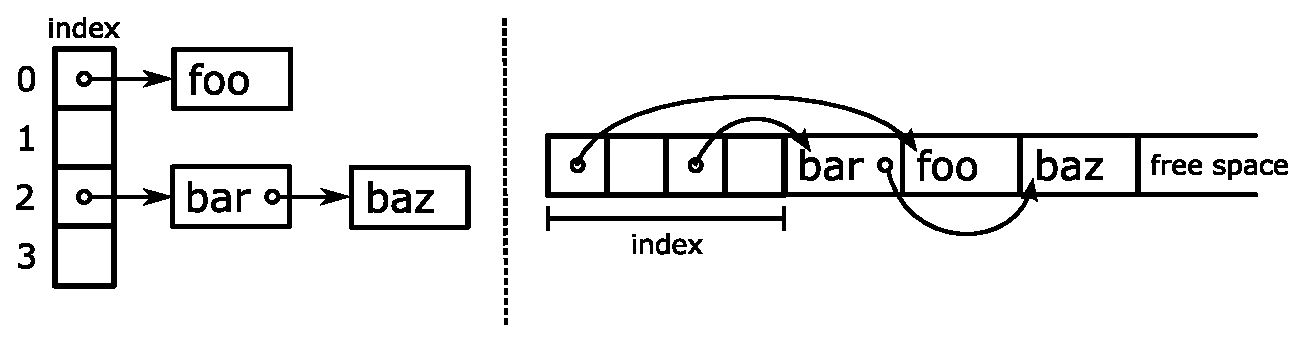
\includegraphics[width=83mm]{hash-table}
\caption{Depiction of a separate-chaining hash table}
\label{fig-hash-table}
\end{figure}

Our hash table implementation uses a fixed size index which must be specified
when creating the hash table, as this simplifies the implementation
considerably. The index is stored at the front of the file, after which values
are simply appended in the order in which they are added. Note that we do not
support removing elements from the hash table, which means we do not have to
deal with holes that would otherwise occur in the stored file.

For our
experiments the FNV-1a hash function \cite{noll2004fnv} is used (modulo the
size of the index) to map values to slots.

\subsubsection{B-tree Implementation}
The B-tree data structure was first proposed by Bayer and McCreight
\cite{bayer1970oam} and is widely implemented and often described in
textbooks. Our implementation is based on the description by Kifer, Bernstein
and Lewis \cite{kifer2006dsa}.

B-trees are similar to other search tree data structures in the sense that
they store ordered values hierarchically in such a way that every subtree stores
consecutive values.
A key property of B-trees is that (unlike most in-memory tree structures) they
do not fix the number of children per node, but instead organize data in pages
of a fixed size, each containing as many values as will fit.
This makes them especially suitable for purposes of on-disk storage where
reading and writing data in a few large blocks is relatively cheap compared to
accessing several smaller blocks.

\begin{figure}[b]
\centering
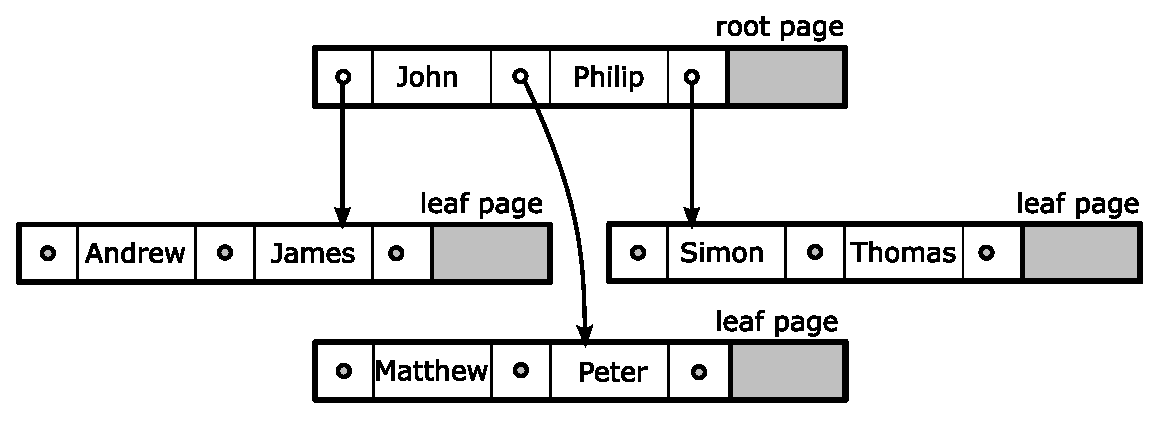
\includegraphics[width=83mm]{b-tree}
\caption{Depiction of a B-tree}
\label{fig-b-tree}
\end{figure}

B-tree pages are ordered in a tree structure. Figure \ref{fig-b-tree} depicts a
B-tree of height two storing eight values.
In each page the values are stored in lexicographical order, and the values
in the first leaf page are lexicographically smaller than ``John'', the values
in the second leaf page are between ``John'' and ``Philip'' and the values in
the third leaf page are greater than ``Philip''. Note that since the page
size is fixed, not all pages are completely filled.

Since every page can store many values, the resulting tree is typically very
shallow, which is beneficial as the number of pages that need to be retrieved
is equal to the height of the tree (worst case).

New values are inserted into a leaf page which can be determined by traversing
the tree.
If this leaf page does not have enough free space to insert the new value,
the page will have to be \emph{split}: the median value is selected, and the old
page is replaced by two new pages containing the values less than respectively
greater than this median value, while the median value itself is moved to the
parent page.
When the top-most page needs to be split, a new (empty) top-level page is
created and the height of the B-tree is increased by one. As a result, all leaf
nodes in a B-tree are at the same depth, and all pages stored are at least half
full, except possibly the root page.

B-trees can easily support the insertion of variable-length values, as long
as each individual value fits in a single page. However, values with
a size larger than the size of a single page must be handled separately.
Our implementation does not support this and therefore requires all
stored values to be smaller than the pages.

\subsubsection{Bender Set Implementation}
\label{sect-bender-set}
The first implementation challenge for the Bender set is that the description
given by Bender et al assumes that all values stored in the set are of a
fixed size, which is not the case in our experimental framework. To work
around this, we create several separate instances of the Bender set with
different value sizes which are powers of two. When a value is to be inserted,
its size is rounded up to a power of two and it is inserted in the
corresponding set instance. This ensures that the amount of space wasted
remains below 50\% while still allowing values of various sizes to be inserted.
The following description will be of a single Bender set instance, and it will
therefore be assumed that values do have a fixed size.

A Bender set has a capacity $C$ that is a power of two. Its implementation
consists of two parts: a sparse array storing the values in order, and a binary
tree stored in van Emde Boas layout that is used to search for values
efficiently.
Both the tree and the array may contain special \emph{empty values}.

Initially, the array stores only empty values and is partitioned into
\emph{windows} on several \emph{levels}.
On the highest level, there is a single window of size $C$. Each subsequent level
has twice as many windows of half that size, and the lowest level has size
$log_2 C$ (rounded up to the next power of 2).
For each level a maximum \emph{density} is chosen, with the lowest level having
density 1, the highest level having density $\delta$, and the density for
the intermediary levels obtained by interpolating linearly between 1 and
$\delta$.

A depiction of a Bender set storing four values (with a capacity for eight) is
given in Figure \ref{fig-bender-set}, with the window population counts for
the sparse array given on the left (density thresholds not shown) and the index
tree on the right.

\begin{figure}
\centering
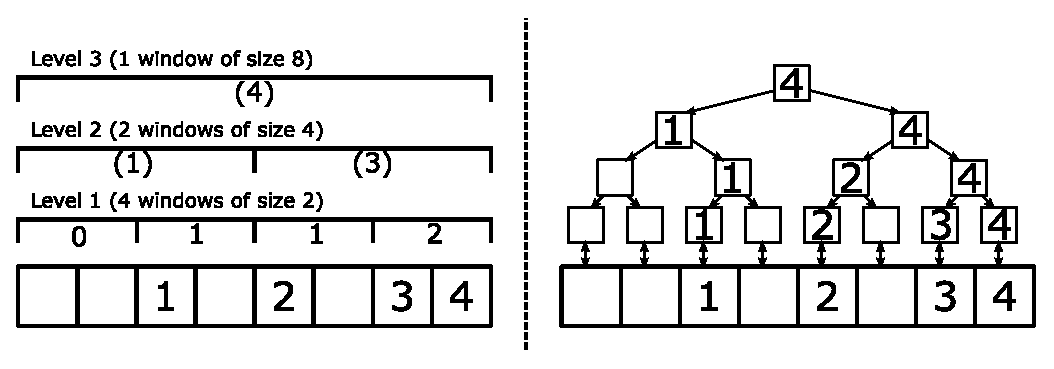
\includegraphics[width=83mm]{bender-set}
\caption{Ddepiction of a Bender set}
\label{fig-bender-set}
\end{figure}

The top-level density must be a number between $0$ and $1$; the optimal value
depends on practical circumstances such as available memory and the relative
cost of rebuilding the data structures.
Whenever the fraction of non-empty values stored in a window (the window's
\emph{population count} divided by the size of the window) exceeds its maximum
density, the window is said to be \emph{overflowing}.
Overflows are resolved when a higher-level window is \emph{rebalanced},
meaning that the values in the window are redistributed evenly over the window,
which will cause some of the values to be moved out of the lower-level windows
which are too full.

To insert a value, the index tree is used to find the position of the smallest
existing value that is greater than the new value (i.e. the value's successor);
the new value will be inserted right before its successor.
Then, the windows overlapping the goal position are considered from bottom to
top. The lowest (smallest) window that can support another element without
overflowing is selected, and then rebalanced (thereby resolving the overflow in
the overlapping lower level windows).

If all windows, including the topmost window spanning the entire array,
would overflow upon insertion of the new element, the capacity of the data
structure must be increased to make room for more elements.
When this happens, the capacity is doubled, a new top level is
created and then the entire array is rebalanced.
Since increasing the capacity causes all values in the array to be moved
and the entire index tree to be recreated, this is an expensive operation;
however, it only occurs infrequently.

According to this description (which follows the paper by Bender et al) a window
is rebalanced every time an element is inserted. As an optimization, our
implementation does not always rebalance a window. When there is free space
between the successor and predecessor of the value to be inserted, the value
is simply inserted in the middle. In our experiments, this optimization
yielded a reduction in execution time.

A detail that is not specified in the paper by Bender et al, is how the
population count for windows is kept. The simplest option is to keep no such
information and simply scan part of the array whenever a population count is
required. Another extreme is to keep population counts for all windows on all
levels, and update these counts whenever values are inserted or moved. In
our experiments a compromise seemed to work best: keep population counts only
for the lowest-level windows, and recompute the counts for higher-level windows
when required. This prevents a lot of recomputation, while keeping the additional
costs of updating low.

Finally, the Bender set uses a complete binary tree as an index data structure
to efficiently find the successor element for a given value. The tree is
stored in memory in van Emde Boas layout to allow cache-oblivious
traversal. This layout is named after the data structure described in
\cite{vanemdeboas1976dai} and determines an order in which the nodes of a
tree can be stored in a contiguous block of memory, in such a way that traversing
a tree with $N$ nodes from root to leaf requires only $O(\log_B N + 1)$ pages to be
fetched from memory.

In van Emde Boas lay-out, which is defined recursively, a tree with 
$N$ nodes is divided in half vertically, creating a small subtree at the
top and a number of subtrees (approximately $\sqrt{N}$) at the bottom.
Each subtree has a size of approximately $\sqrt{N}$ nodes and is stored in
van Emde Boas layout in a contiguous block of memory; these blocks are then
stored consecutively.

In Figure \ref{fig-van-emde-boas} a binary tree is shown, with the nodes
labeled with their positions according to the van Emde Boas layout.
In this example, only two levels of recursion are needed. If we suppose that
every page stores three nodes, then the highlighted path from node 1 to 12
visits only two pages.

\begin{figure}
\centering
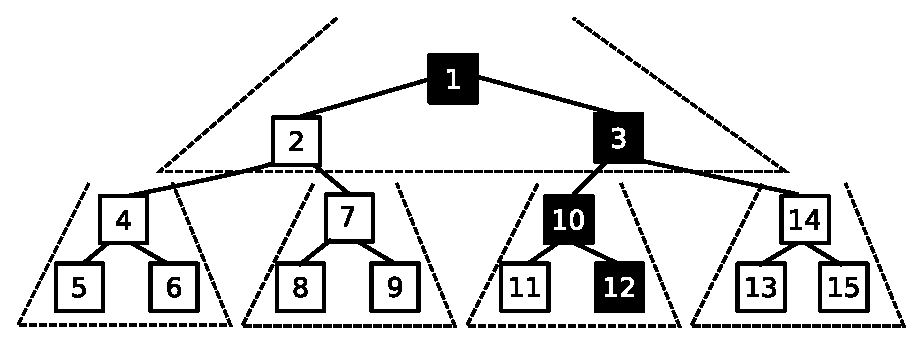
\includegraphics[width=83mm]{vanemdeboas}
\caption{A binary tree in van Emde Boas layout}
\label{fig-van-emde-boas}
\end{figure}

In the index tree used for the Bender set, the leaf nodes store the same values
as the sparse array (including empty values).
Interior nodes store the maximum value of their two children (or an empty value,
if both children store an empty value).
This tree can be used in a similar way as a binary search tree: by examining the
two children of a node, we can determine whether a searched-for value belongs
in the left or right subtree.
See the right side of Figure \ref{fig-bender-set} for an example.

Note that the \emph{structure} of the tree is static and only changes when the
capacity of the set is increased (in which case the tree is recreated from scratch).
Of course, the values stored in the tree have to be updated when the corresponding
elements of the array change.

\subsection{Measurements}
Measuring the memory usage of a process can be done by retrieving how much of the
address space has been allocated by a process; called the \emph{virtual set
size}. This does not necessarily correspond one-to-one with memory being allocated
for the process, but since the majority of the memory used by the
data structures is mapped at exactly one location, this metric is suitable
for our experiments.

There are several ways of measuring the time a process takes to execute.
The simplest is counting the number of seconds elapsed since the start of the
program (called \emph{wall clock time}).
This has the disadvantage that concurrently executing processes affect the timing
of the process being measured, so on a busy system the reported time may vary
over different executions.

A different way to measure time is using the statistics the kernel collects
of how many seconds the processor spends executing instructions for the process
(both in user space and in kernel space). These values are independent of
what other processes are doing, which makes them more consistent across
multiple executions. However, these values do not account for the time the
system spends waiting (for example, for data to be read from disk)
or the time spent by other processes on behalf of the executing process
(for example, the kernel swap daemon on Linux). Since these factors may have
a large effect on the total running time of the algorithm, it is undesirable
to leave these out.

Therefore, we decided to measure wall clock time and deal with variations
across multiple executions by running each experiment seven times and using
the median value for further analysis.

\subsubsection{Framework Overhead}
Finally, there is another factor that must be taken into account: the test
framework uses several components (such as the NIPS VM and a queue) that are
not being evaluated, yet which do contribute to the memory use and runtime
of the process. In order to discount these factors, tests are performed using
a mock set implementation that gives a near-minimal overhead. This works
by first running with a real set implementation and logging all results
(the return values of the \verb#insert(S,x)# calls) to a file, and then
running a second time while reading the stored values. In the second run,
the mock set implementation does not have to actually store or retrieve
data and consequently has negligible memory and runtime overhead.

In the results below, all values are reported relative to the values obtained
using the mock set implementation, which means the overhead of the test
framework is removed from the results. Although the extra memory used by
the test framework is relatively small (less than 10\% in all cases) and
primarily caused by the queue data structure, the overhead in terms of
execution time was quite significant: close to 70\% on the worst case.
This does mean that the set data structure accounts for at least 30\%
of the execution time of the search algorithm in all cases (and much
more for the slower data structures).

\subsubsection{System Configuration}
The experiments where performed on a 64-bit Linux system (kernel version 2.6.18)
with an Intel Xeon E5335 processor (2~GHz, 4~MB cache) and 8~GB of main
memory (no swap file). Although the system is a multiprocessor system
(and the E5335 is a dual-core processor) all code is single-threaded so
only a single core is used when executing tests.

The following models are used for benchmarking:
\begin{itemize}
\item\textbf{Eratosthenes} is a parallel implementation of the sieve
of Eratosthenes which is used to find prime numbers up to a given maximum.
It has a single parameter $N$: only integers from 2 to $N$ (exclusive) are
tested. A new process is created for every prime number found, and as a result
the state space can only be exhaustively searched for relatively small values
of $N$ (e.g. $N < 40$). Because processes are dynamically created, state size
increases during execution.

\item\textbf{Leader2} is a leader election algorithm with a configurable number
of processes competing for leadership ($N$). Since a constant number of
processes will be created and these processes cannot make progress until all
of them are created, almost all states have the same size.

\item\textbf{Peterson\_N} is Peterson's solution to the multi-process mutual
exclusion problem (using global variables instead of channels for
communication) with a configurable number of processes ($N$). The processes
are created atomically, so the state size is constant after initialization.
\end{itemize}

\begin{table}
\begin{center}
\begin{tabular}{ l l r r }
\hline
\textbf{Model} & \textbf{Parameters} & \textbf{Iterations} & \textbf{Transitions} \\
\hline
Eratosthenes & $N=40$ &  1,019,960 &  4,923,218 \\
Leader2      & $N=5$  &  5,950,945 & 23,856,363 \\
Peterson\_N  & $N=4$  & 10,000,000 & 37,434,411 \\
\hline
\end{tabular}
\caption{Properties of test cases used}
\label{tab-cases}
\end{center}
\end{table}

% TODO: add state sizes to table?

In Table \ref{tab-cases} an overview is given of the parameters of the models used
and the resulting properties of the state space search.
Note that the number of transitions relative to the number of iterations gives an
indication of the ratio of value look-ups (insertions of values that are already
present in the set) and actual insertions, ranging approximately from 4 to
2.7 look-ups per insertion.

% Possible additional cases:
% - mobile1
% - pftp
% - snoopy
% - sort

\section{Results}
Each of the tree data structures has some configurable parameters. The hash table
needs to be parametrized with the size of the index, the B-tree with the size of
the pages, and the Bender set with the density parameter ($\delta$). To determine
which parameters to use, various different parameters were first tried on the
first (and smallest) test case. In this case, a million relatively small states
need to be stored.

Figure \ref{fig-eratosthenes-hash_wctime} shows the execution times for the hash
table.
The hash table
with a small index (100,000 slots) performs well initially, but gets slower as
it becomes too full, at which point each slot in the hash table has to store a
long list of values that map to that slot.
As Figure \ref{fig-eratosthenes-hash_vss} shows, the only difference in memory
usage of the different hash tables is in the (fixed) size of the index.
We will use the hash table with an index size of 10 million slots for further
experiments, as it performed best in this case, and seems suitable for other
cases (which require storing more values) as well.

Figure \ref{fig-eratosthenes-btree_wctime} and Figure
\ref{fig-eratosthenes-btree_vss} show the execution time and memory usage
for the B-tree with page sizes ranging from 1~kilobyte to 16~kilobyte.
The execution platform
maps memory in 4~KB pages, which would suggest that using pages less than 4~KB
makes little sense. Indeed, the B-tree with 1~KB pages seems to perform worst,
but if we take the memory use into account, this is most likely due to the fact
that fewer items fit on a single page, which means a relatively large portion of
the page remains unused.
The difference between 4~KB and 16~KB pages is relatively small (both in
execution time and memory usage); we select the 16~KB page size for further
experiments because state sizes are larger in other test cases, in which case
the 4~KB page size may cause similar problems as the 1~KB page size here.

Finally, in Figure \ref{fig-eratosthenes-bender_wctime} the execution times for
the Bender set with several different density parameters are given. With a lower
density, more space is required, but new insertions less frequently cause large windows to be rebalanced.
The execution times for the density values of 0.5 and lower are almost the same
while larger density values are slower.
Figure \ref{fig-eratosthenes-bender_vss} shows that the lower the density value,
the more memory is used. It appears that the advantage of low density is
negated by the overhead of constructing increasingly large data structures.
The set with $\delta=0.125$ cannot even finish the test case in the memory
that is available. We select $\delta=0.5$ for future experiments, which strikes
a good balance between execution time and memory requirements.

Now that we have established the parameters to use for the other test cases,
we can run final experiments on all three test cases.
The execution times for these cases are presented in Figure \ref{fig-wctime}
and the corresponding memory usage is presented in Figure \ref{fig-vss}.

\section{Discussion}
The three test cases paint a very similar picture: in all cases, the hash table
offers the best performance in terms of both execution time and memory usage,
followed by the B-tree. In all cases, the Bender set performs worst by a large
margin.

It should be noted that the Bender set is the only data structure that shows
abrupt changes in both the execution time and memory usage graphs. These
jumps in the graph occur whenever the capacity of the Bender set is increased;
this causes the memory allocated for the set to be doubled and the array and
tree structures to be recreated, which is a relatively expensive operation.

The difference in execution time between the hash table and B-tree increases as
the size of the states becomes larger. This is explained by the fact that the
height of the B-tree depends on the average number of values per page; larger
values means less values per page, and therefore a deeper tree, and as a
result more pages to be fetched for a query. The hash table does not have such a
limitation, as every value in the bucket must be fetched independently, regardless
of the size of these values.

With respect to memory usage the B-tree and hash table have similar requirements;
the B-tree has slightly larger overhead per value stored, but initially the hash
table uses more memory because of the space allocated for the index.

The performance of the Bender set does not seem to depend on the page size,
and as a result the difference between the Bender set and the B-tree is smallest
when the page size is largest. Unfortunately, even then it requires about three
times as much time (and 5--6 times as much memory).

The increased memory requirements of the Bender set can in part be explained by
our implementation of variable-length values, which wastes some space by storing
them in fixed-size slots. This overhead should be around 25\% on average.

The test cases used all have a relatively high ratio of value insertions to
look-ups. This may explain the good performance of the hash table (for
which insertions are barely more expensive than look-ups) as well as the bad
performance of the Bender tree (for which insertions are relatively expensive,
especially when a window is rebalanced). Unfortunately, our experiments do not
give enough data to determine how the relative performance of the data
structures changes when this ratio changes.

\subsection{Implementation Complexity}
Since all data structures included in the experiments were implemented from
scratch, our research also yields some insight in the implementation complexity
of the different data structures.

Table \ref {tab-loc} gives the number of lines of source code used to implement
various part of the test application, after removing comments and blank lines
(which amount to about 25\% of the code).
Common code includes allocation functions, interface descriptions and comparison
and hashing functions. The framework includes not just the search algorithm,
but also the functionality to report various metrics while running a test case.

\begin{table}[t]
\begin{center}
\begin{tabular}{ l r r }
\hline
\textbf{Purpose} & \textbf{Lines} & \textbf{Percentage} \\
\hline
Common code       & 433 & 18.21\% \\
Hash table        & 146 &  6.14\% \\
B-tree            & 299 & 12.57\% \\
Bender set        & 623 & 26.20\% \\
Queue             & 184 &  7.74\% \\
Search Framework  & 693 & 29.14\% \\
\hline
\end{tabular}
\caption{Source lines of code of the test application}
\label{tab-loc}
\end{center}
\end{table}

Although not a perfect metric of implementation complexity, the lines of code
required for the various components of the test application do give some
insight in the relative complexity of the data structures. It is clear why
hash tables are a popular choice: they are easy to implement yet perform very
well. The Bender set not only uses more lines of code, but in our experience
also required a greater amount of effort to implement correctly.

\section{Future Work}
It should be noted that in our experiments only part of the memory
hierarchy was used (up to the use of main memory). This still involves several
levels of processor cache, but it is not a very deep hierarchy. In a deeper
memory hierarchy, with greater differences in access times between the levels,
the cache-efficient data structures (the B-tree and the Bender set) should
perform better. Specifically, using disk-based storage as the lowest level of
storage seems a logical extension of our research.

In our experiments we did not measure cache efficiency specifically; instead,
we measured total execution time only, which is affected by several different
factors of which cache efficiency is only one.
To better understand how different factors influence performance, it would
be interesting to measure cache efficiency separately and report on actual
cache hits and misses on different boundaries of the memory hierarchy.

Finally, we only evaluated a single data structure in a single test
environment (even though we used more than one model to perform experiments).
To draw more general conclusions about the practical merits of cache-oblivious
data structures, it will be necessary to perform experiments at a larger scale,
comparing multiple cache-oblivious data structures and using scenarios that
differ more.

\section{Conclusion}
The experimental results clearly show that the cache-oblivious data structure
proposed by Bender, Duan, Iacono and Wu is outperformed by traditional data
structures in our test scenario, in terms of both execution time and memory use.
The advantage of more cache-friendly behavior does not appear to be large enough
to compensate for the increased complexity of the data structure, which results in
higher memory requirements and increased computational overhead.
If the data structure does have asymptotic performance benefits, then realistic
work loads on current hardware systems are not enough to reveal this.
These findings are consistent with earlier results, such as obtained by
Rahman, Cole and Raman, and Olsen and Skov (see Section \ref{sect-related-work}).

Of course, this does not prove conclusively that cache-oblivious data structures
are entirely without merit. Our experiments are limited in scope: only a single
cache-oblivious data structure has been examined, in a single test scenario,
on a single platform.
In a different setting, different cache-oblivious data structures might compare
favorably to their traditional counterparts.
However, since the observed differences in performance are fairly large,
it is unlikely that small changes are enough to close the performance gap.

We hope that future research on cache-oblivious data structures will not focus
on theoretical performance alone, but will also compare performance in practice
with existing alternatives.
Although theoretical results are invaluable, newly developed data structures and
algorithms should, preferably, have demonstrable practical merit as well.

\bibliographystyle{unsrt}
\bibliography{paper}

\begin{figure*}[p]
\centering
\subfigure[B-tree]{
    \label{fig-eratosthenes-hash_wctime}
    \includegraphics[width=56mm]{fig-eratosthenes-hash_wctime}}
\subfigure[Hash table]{
    \label{fig-eratosthenes-btree_wctime}
    \includegraphics[width=56mm]{fig-eratosthenes-btree_wctime}}
\subfigure[Bender set]{
    \label{fig-eratosthenes-bender_wctime}
    \includegraphics[width=56mm]{fig-eratosthenes-bender_wctime}}
\caption{Execution times per data structure on Eratosthenes}
\label{fig-eratosthenes-wctime}
\end{figure*}

\begin{figure*}[p]
\centering
\subfigure[B-tree]{
    \label{fig-eratosthenes-hash_vss}
    \includegraphics[width=56mm]{fig-eratosthenes-hash_vss}}
\subfigure[Hash table]{
    \label{fig-eratosthenes-btree_vss}
    \includegraphics[width=56mm]{fig-eratosthenes-btree_vss}}
\subfigure[Bender set]{
    \label{fig-eratosthenes-bender_vss}
    \includegraphics[width=56mm]{fig-eratosthenes-bender_vss}}
\caption{Memory usage per data structure on Eratosthenes}
\label{fig-eratosthenes-vss}
\end{figure*}

\begin{figure*}[p]
\centering
\subfigure[Eratosthenes]{
    \label{fig-eratosthenes_wctime}
    \includegraphics[width=56mm]{fig-eratosthenes_wctime}}
\subfigure[Leader2]{
    \label{fig-leader2_wctime}
    \includegraphics[width=56mm]{fig-leader2_wctime}}
\subfigure[Peterson\_N]{
    \label{fig-peterson_wctime}
    \includegraphics[width=56mm]{fig-peterson_wctime}}
\caption{Execution times per test case}
\label{fig-wctime}
\end{figure*}

\begin{figure*}[p]
\centering
\subfigure[Eratosthenes]{
    \label{fig-eratosthenes_vss}
    \includegraphics[width=56mm]{fig-eratosthenes_vss}}
\subfigure[Leader2]{
    \label{fig-leader2_vss}
    \includegraphics[width=56mm]{fig-leader2_vss}}
\subfigure[Peterson\_N]{
    \label{fig-peterson_vss}
    \includegraphics[width=56mm]{fig-peterson_vss}}
\caption{Memory usage per test case}
\label{fig-vss}
\end{figure*}

\end{document}
